\chapter{Конструкторская часть}
В данном разделе будут рассмотрены требования к программе и алгоритмы визуализации сцены и молнии.


\section{Требования к программе}
Программа должна предоставлять следующие возможности:
\begin{itemize}
	\item визуальное отображение сцены;
	\item запуск и остановка ударов молнии;
	\item возможность включения и выключения света во всех окнах дома;
	\item поворот исходной сцены.
\end{itemize}


\section{Общий алгоритм решения поставленной задачи}
\begin{enumerate}
	\item Задать объекты сцены (дом, окна, в которых включен свет).
	\item Задать частоту обновления количества окон, в которых включен свет.
	\item Рассчитать координаты конца молнии, и в зависимости от этого рассчитать куда ударит молния.
	\begin{enumerate}
		\item Если конец молнии находится в области дома, то молния ударит в молниезащиту дома.
		\item Если конец молнии находится вне области дома, то молния ударит в землю в случае, если молния-лидер.
	\end{enumerate}
	\item Изобразить молнию.
\end{enumerate}


\section{Алгоритм обратной трассировки лучей}

Алгоритмы трассировки лучей на сегодняшний день считаются наиболее мощными при создании реалистичных изображений. 

Изображение формируется из-за того, что свет попадает в камеру. Выпустим из источников света множество лучей (первичные лучи). Часть этих лучей “улетит” в свободное пространство, а часть попадет на объекты. На них лучи могут преломляться и отражаться. При этом часть энергии луча поглотится. Преломленные и отраженные лучи образуют новое поколение лучей. Далее эти лучи опять же преломятся, отразятся и образуют новое поколение лучей. В конечном итоге часть лучей попадет в камеру и сформирует изображение. Это описывает работу прямой трассировки лучей.

Метод обратной трассировки лучей позволяет значительно сократить перебор световых лучей. В этом методе отслеживаются лучи не от источников, а из камеры. Таким образом, трассируется определенное число лучей, равное разрешению картинки \cite{raytrace}.   

\img{90mm}{tracric}{Пример работы алгоритма трассировки лучей}
 
Пусть есть камера и экран, находящийся на расстоянии h от камеры (рисунок \ref{img:tracric}). Для удобства следует разбить экран на квадраты. Далее по очереди необходимо проводить лучи из камеры в центр каждого квадрата (первичные лучи). После этого надо найти пересечение каждого такого луча с объектами сцены и выбрать среди всех пересечений самое близкое к камере. Далее, применив нужную модель освещения, можно получить изображение сцены. Это самый простой метод обратной трассировки лучей. Он позволяет лишь отсечь невидимые грани.

Но если надо смоделировать такое явление как отражение, то необходимо из самого близкого пересечения пустить вторичные лучи. Например, если поверхность отражает свет, и она идеально ровная, то необходимо отразить первичный луч от поверхности и пустить по этому направлению вторичный луч. Если же поверхность неровная, то необходимо пустить множество вторичных лучей. 

На рисунке \ref{img:trac} представлена схема алгоритма.

\img{150mm}{trac}{Схема алгоритма трассировки лучей}

\clearpage

\section{Способ оптимизации алгоритма трассировки лучей}
Для уменьшения времени работы алгоритма при реализации данной программы необходимо испускать лучи из камеры не по всей сцене, а в отдельные ее участки. Во-первых, лучи пускаются во все сегменты молнии для того, чтобы узнать, где находится молния за домом или перед ним. Во-вторых, лучи пускаются в черные окна, чтобы затем пустить из них вторичный луч и понять отражается в них молния или нет. Таким образом можно получить большой выигрыш по времени.

\section{Алгоритм генерации молнии}
Первоначально случайным образом задаются две координаты на молнии, ее конец и начало. По данным двум точками строится прямая, путем вычитания из координат конца координаты начала молнии, также находим расстояние от нее до громоотвода. Если расстояние это меньше нужного, то нужно поменять координаты конца на координаты вершины громоотвода.

Существует два вида молнии.
\begin{enumerate}
	\item Обычная молния -- это молния, которая не доходит до объекта или земли (рисунок \ref{img:m1}).
	\item Молния-лидер -- это молния, которая доходит до какого-то объекта либо до земли (рисунок \ref{img:m2}). 
\end{enumerate}

\begin{figure}[h!]
	\begin{center}
		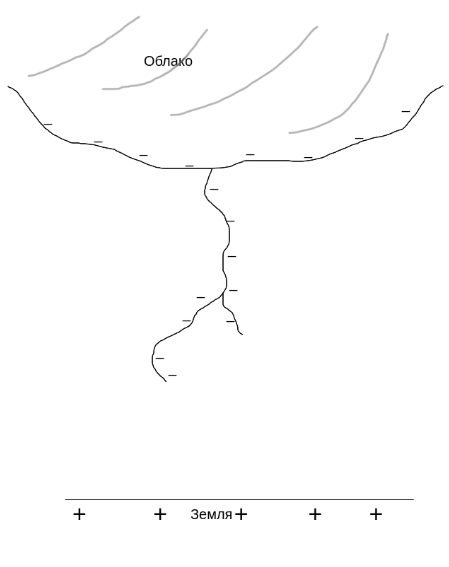
\includegraphics[scale=0.48]{img/m1.png}
	\end{center}
	\captionsetup{justification=centering}
	\caption{Обычная молния}
	\label{img:m1}
\end{figure}

\begin{figure}[H]
	\begin{center}
		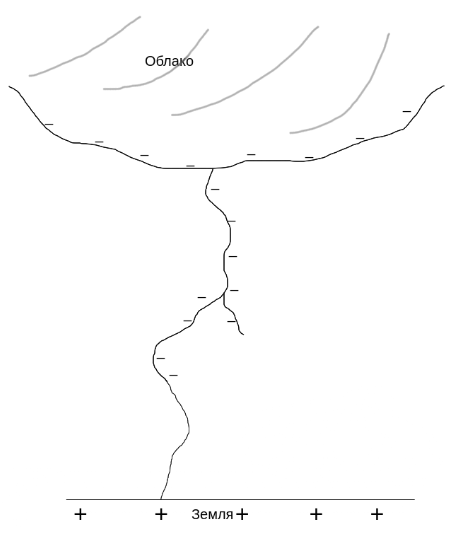
\includegraphics[scale=0.48]{img/m2.png}
	\end{center}
	\captionsetup{justification=centering}
	\caption{Молния-лидер}
	\label{img:m2}
\end{figure}



Далее генерацию молнии можно разделить на два случая.
\begin{enumerate}
	\item Молния бьет в землю – в данном случае молния имеет более непредсказуемый характер и может себя вести произвольно.
	\item Молния бьет в громоотвод – в данном случае молния движется от начала удара до вершины громоотвода с небольшими колебаниями.
\end{enumerate}

Каждую итерацию каждый сегмент делится пополам, с небольшим сдвигом центральной точки.

Чтобы создать ветви, когда разделяем сегмент молнии, вместо добавления двух сегментов надо добавить три. Третий сегмент – это продолжение молнии в направлении первого с небольшим отклонением.

На каждом сегменте с вероятностью в 1\% появляется побочная ветвь, которая строится по таким же законам, как и главная в том случае, если молния бьет в землю. Для каждой такой побочной ветви генерируется угол на который она повернута относительно главной ветви. Длина побочного сегмента зависит от того, в каком месте молнии она появляется: чем ближе к концу, тем короче она будет. 

Пример генерации молнии без побочных сегментов (ветвей) представлен на рисунке \ref{img:moln1} и с побочными сегментами (ветвями) -- на рисунке \ref{img:moln2}.

\img{30mm}{moln1}{Генерация молнии без побочных ветвей}

\img{40mm}{moln2}{Генерация молнии с побочными ветвями}

\section{Модель освещения Ламберта}

Данная модель вычисляет цвет поверхности в зависимости от того как на нее светит источник света. Согласно данной модели, освещенность точки равна произведению силы источника света и косинуса угла, под которым он светит на точку \cite{lamber_fong}.

\begin{equation}
	\label{eq:lambert}
	I_{d} = k_{d}  cos(L, N)  i_{d},
\end{equation}
где:
\begin{itemize}
	\item $I_{d}$ -- рассеянная составляющая освещенности в точке;
	\item $k_{d}$ -- свойство материала воспринимать рассеянное освещение;
	\item $i_{d}$ -- мощность рассеянного освещения;
	\item $L$ -- направление из точки на источник;
	\item $N$ -- вектор нормали.
\end{itemize}

\section{Генерация дома}
Дом удобнее генерировать с помощью массива точек, ограничивающих сторону дома.

Дом состоит из 5 объектов – 4 стороны и крыша. Они задаются путем задания координат для каждой стороны. Для каждой координаты задается три параметра – координаты $X$, $Y$, $Z$. Высота дома зависит от этажности. После задания данных параметров создаются и накладываются окна. 

Каждое окно, как и сторона дома, ограничено массивом точек. Для каждого окна задаются ограничивающие его 4 точки. Задаются они путём задания трёх координат для каждой стороны. В зависимости от количества этажей создаются окна. На каждый этаж приходится по 8 окон. 

Также создается громоотвод (молниезащита дома). 

\section{Выбор используемых типов и структур данных}

Для разрабатываемого ПО необходимо реализовать следующие типы и структуры данных.
\begin{enumerate}
	\item Сцена - список объектов.
	\item Объекты сцены - набор вершин и граней.
	\item Источник света - положение и направление света.
	\item Цвет - вектор из трех числе (синий, красный, зеленый).
	\item Математические абстракции:
	\begin{enumerate}
		\item точка - хранит положение, задается координатами $x$, $y$, $z$;
		\item вектор - хранит направление, задается  $x$, $y$, $z$;
		\item многоугольник - хранит вершины, нормаль, цвет.
	\end{enumerate}
\end{enumerate}


\section{Вывод}
В данном разделе были описаны требования к программе, подробно рассмотрены алгоритмы, которые будут реализованы, и приведена схема алгоритма трассировки лучей, а также указан способ оптимизации данного алгоритма для поставленной задачи.
